\documentclass{book}


% required packages
\usepackage{Sweave}
\usepackage{Zelig}\usepackage{Zinput}


% begin body
\begin{document}


\chapter{Normal Regression for Continuous Dependent Variables}

\nobibliography*

\section{{\tt normal}: Normal Regression for Continuous Dependent Variables}
\label{normal}

The Normal regression model is a close variant of the more standard
least squares regression model (see \Sref{ls}). Both models specify a
continuous dependent variable as a linear function of a set of
explanatory variables.  The Normal model reports maximum likelihood
(rather than least squares) estimates.  The two models differ only in
their estimate for the stochastic parameter $\sigma$.

\subsubsection{Syntax}

\begin{verbatim}
> z.out <- zelig(Y ~ X1 + X2, model = "normal", data = mydata)
> x.out <- setx(z.out)
> s.out <- sim(z.out, x = x.out)
\end{verbatim}

\subsubsection{Additional Inputs} 

In addition to the standard inputs, {\tt zelig()} takes the following
additional options for normal regression:  
\begin{itemize}
\item {\tt robust}: defaults to {\tt FALSE}.  If {\tt TRUE} is
selected, {\tt zelig()} computes robust standard errors via the {\tt
sandwich} package (see \cite{Zeileis04}).  The default type of robust
standard error is heteroskedastic and autocorrelation consistent (HAC),
and assumes that observations are ordered by time index.

In addition, {\tt robust} may be a list with the following options:  
\begin{itemize}
\item {\tt method}:  Choose from 
\begin{itemize}
\item {\tt "vcovHAC"}: (default if {\tt robust = TRUE}) HAC standard
errors. 
\item {\tt "kernHAC"}: HAC standard errors using the
weights given in \cite{Andrews91}. 
\item {\tt "weave"}: HAC standard errors using the
weights given in \cite{LumHea99}.  
\end{itemize}  
\item {\tt order.by}: defaults to {\tt NULL} (the observations are
chronologically ordered as in the original data).  Optionally, you may
specify a vector of weights (either as {\tt order.by = z}, where {\tt
z} exists outside the data frame; or as {\tt order.by = \~{}z}, where
{\tt z} is a variable in the data frame).  The observations are
chronologically ordered by the size of {\tt z}.
\item {\tt \dots}:  additional options passed to the functions 
specified in {\tt method}.   See the {\tt sandwich} library and
\cite{Zeileis04} for more options.   
\end{itemize}
\end{itemize}

\subsubsection{Examples}

\begin{enumerate}
\item Basic Example with First Differences

Attach sample data: 
\begin{Schunk}
\begin{Sinput}
> data(macro)
\end{Sinput}
\end{Schunk}
Estimate model:  
\begin{Schunk}
\begin{Sinput}
> z.out1 <- zelig(unem ~ gdp + capmob + trade, model = "normal", 
+     data = macro)
\end{Sinput}
\end{Schunk}
Summarize of regression coefficients:  
\begin{Schunk}
\begin{Sinput}
> summary(z.out1)
\end{Sinput}
\end{Schunk}
Set explanatory variables to their default (mean/mode) values, with
high (80th percentile) and low (20th percentile) values for trade: 
\begin{Schunk}
\begin{Sinput}
> x.high <- setx(z.out1, trade = quantile(macro$trade, 0.8))
> x.low <- setx(z.out1, trade = quantile(macro$trade, 0.2))
\end{Sinput}
\end{Schunk}
Generate first differences for the effect of high versus low trade on
GDP: 
\begin{Schunk}
\begin{Sinput}
> s.out1 <- sim(z.out1, x = x.high, x1 = x.low)
\end{Sinput}
\end{Schunk}
\begin{Schunk}
\begin{Sinput}
> summary(s.out1)
\end{Sinput}
\end{Schunk}
%plot does not work 
A visual summary of quantities of interest:  
\begin{center}
\begin{Schunk}
\begin{Sinput}
> plot(s.out1)
\end{Sinput}
\end{Schunk}
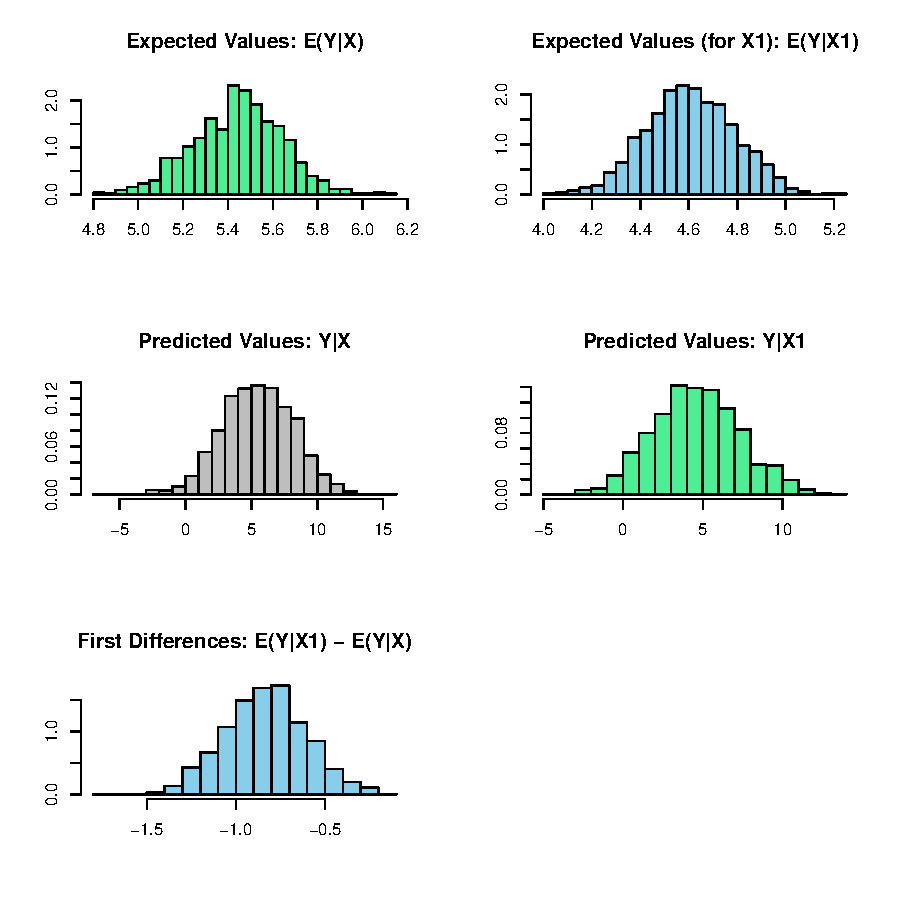
\includegraphics{vigpics/normal-ExamplesPlot}
\end{center}

\item Using Dummy Variables
%the code in this section does not work well but there is no demo for this part either
 
Estimate a model with a dummy variable for each year and country (see
\ref{factors} for help with dummy variables).  Note that you do not
need to create dummy variables, as the program will automatically
parse the unique values in the selected variables into dummy
variables.    
\begin{Schunk}
\begin{Sinput}
> z.out2 <- zelig(unem ~ gdp + trade + capmob + as.factor(year) + 
+     as.factor(country), model = "normal", data = macro)
\end{Sinput}
\end{Schunk}
Set values for the explanatory variables, using the default mean/mode
variables, with country set to the United States and Japan,
respectively: 
Simulate quantities of interest:  
%plot does not work 
\begin{center}
\end{center}
\end{enumerate}

\subsubsection{Model}
Let $Y_i$ be the continuous dependent variable for observation $i$.
\begin{itemize}
\item The \emph{stochastic component} is described by a univariate normal
  model with a vector of means $\mu_i$ and scalar variance $\sigma^2$:
  \begin{equation*}
    Y_i \; \sim \; \textrm{Normal}(\mu_i, \sigma^2). 
  \end{equation*}

\item The \emph{systematic component} is 
  \begin{equation*}
    \mu_i \;= \; x_i \beta,
  \end{equation*}
  where $x_i$ is the vector of $k$ explanatory variables and $\beta$ is
  the vector of coefficients.
\end{itemize}


\subsubsection{Quantities of Interest}

\begin{itemize}
\item The expected value ({\tt qi\$ev}) is the mean of simulations
  from the the stochastic component, $$E(Y) = \mu_i = x_i \beta,$$
  given a draw of $\beta$ from its posterior.  

\item The predicted value ({\tt qi\$pr}) is drawn from the distribution
  defined by the set of parameters $(\mu_i, \sigma)$.  

\item The first difference ({\tt qi\$fd}) is:
\begin{equation*}
\textrm{FD}\; = \;E(Y \mid x_1) -  E(Y \mid x)
\end{equation*}

\item In conditional prediction models, the average expected treatment
  effect ({\tt att.ev}) for the treatment group is 
    \begin{equation*} \frac{1}{\sum_{i=1}^n t_i}\sum_{i:t_i=1}^n \left\{ Y_i(t_i=1) -
      E[Y_i(t_i=0)] \right\},
    \end{equation*} 
    where $t_i$ is a binary explanatory variable defining the treatment
    ($t_i=1$) and control ($t_i=0$) groups.  Variation in the
    simulations are due to uncertainty in simulating $E[Y_i(t_i=0)]$,
    the counterfactual expected value of $Y_i$ for observations in the
    treatment group, under the assumption that everything stays the
    same except that the treatment indicator is switched to $t_i=0$.

\item In conditional prediction models, the average predicted treatment
  effect ({\tt att.pr}) for the treatment group is 
    \begin{equation*} \frac{1}{\sum_{i=1}^n t_i}\sum_{i:t_i=1}^n \left\{ Y_i(t_i=1) -
      \widehat{Y_i(t_i=0)} \right\},
    \end{equation*} 
    where $t_i$ is a binary explanatory variable defining the
    treatment ($t_i=1$) and control ($t_i=0$) groups.  Variation in
    the simulations are due to uncertainty in simulating
    $\widehat{Y_i(t_i=0)}$, the counterfactual predicted value of
    $Y_i$ for observations in the treatment group, under the
    assumption that everything stays the same except that the
    treatment indicator is switched to $t_i=0$.

\end{itemize}

\subsubsection{Output Values}

The output of each Zelig command contains useful information which you
may view.  For example, if you run \texttt{z.out <- zelig(y \~\,
  x, model = "normal", data)}, then you may examine the available
information in \texttt{z.out} by using \texttt{names(z.out)},
see the {\tt coefficients} by using {\tt z.out\$coefficients}, and
a default summary of information through \texttt{summary(z.out)}.
Other elements available through the {\tt \$} operator are listed
below.

\begin{itemize}
\item From the {\tt zelig()} output object {\tt z.out}, you may extract:
   \begin{itemize}
   \item {\tt coefficients}: parameter estimates for the explanatory
     variables.
   \item {\tt residuals}: the working residuals in the final iteration
     of the IWLS fit.
   \item {\tt fitted.values}: fitted values.  For the normal model,
     these are identical to the {\tt linear predictors}.
   \item {\tt linear.predictors}: fitted values.  For the normal
     model, these are identical to {\tt fitted.values}.
   \item {\tt aic}: Akaike's Information Criterion (minus twice the
     maximized log-likelihood plus twice the number of coefficients).
   \item {\tt df.residual}: the residual degrees of freedom.
   \item {\tt df.null}: the residual degrees of freedom for the null
     model.
   \item {\tt zelig.data}: the input data frame if {\tt save.data = TRUE}.  
   \end{itemize}

\item From {\tt summary(z.out)}, you may extract: 
   \begin{itemize}
   \item {\tt coefficients}: the parameter estimates with their
     associated standard errors, $p$-values, and $t$-statistics.
   \item{\tt cov.scaled}: a $k \times k$ matrix of scaled covariances.
   \item{\tt cov.unscaled}: a $k \times k$ matrix of unscaled
     covariances.  
   \end{itemize}

\item From the {\tt sim()} output object {\tt s.out}, you may extract
  quantities of interest arranged as matrices indexed by simulation
  $\times$ {\tt x}-observation (for more than one {\tt x}-observation).
  Available quantities are:

   \begin{itemize}
   \item {\tt qi\$ev}: the simulated expected values for the specified
     values of {\tt x}.
   \item {\tt qi\$pr}: the simulated predicted values drawn from the
     distribution defined by $(\mu_i, \sigma)$.
   \item {\tt qi\$fd}: the simulated first difference in the simulated
     expected values for the values specified in {\tt x} and {\tt x1}.
   \item {\tt qi\$att.ev}: the simulated average expected treatment
     effect for the treated from conditional prediction models.  
   \item {\tt qi\$att.pr}: the simulated average predicted treatment
     effect for the treated from conditional prediction models.  
   \end{itemize}
\end{itemize}

\subsection* {How to Cite} 

How to cite this model in Zelig:
\begin{verse}
  Kosuke Imai, Gary King, and Olivia Lau. 2008. "normal: Normal Regression for Continuous Dependent Variables" in Kosuke Imai, Gary King, and Olivia Lau, "Zelig: Everyone's Statistical Software,"http://gking.harvard.edu/zelig
\end{verse}

\CiteZelig

\subsection* {See also}

The normal model is part of the stats package by \citet{VenRip02}.
Advanced users may wish to refer to \texttt{help(glm)} and
\texttt{help(family)}, as well as \cite{McCNel89}. Robust standard
errors are implemented via the sandwich package by \citet{Zeileis04}.
Sample data are from \cite{KinTomWit00}.

\bibliographystyle{asa}
\bibliography{gk,gkpubs}
 



\chapter{Least Squares Regression for Continuous Dependent Variables}

\nobibliography*


\section{{\tt ls}: Least Squares Regression for Continuous
Dependent Variables}
\label{ls}

Use least squares regression analysis to estimate the best linear
predictor for the specified dependent variables.

\subsubsection{Syntax}

\begin{verbatim}
> z.out <- zelig(Y ~ X1 + X2, model = "ls", data = mydata)
> x.out <- setx(z.out)
> s.out <- sim(z.out, x = x.out)
\end{verbatim}

\subsubsection{Additional Inputs}  

In addition to the standard inputs, {\tt zelig()} takes the following
additional options for least squares regression:  
\begin{itemize}
\item {\tt robust}: defaults to {\tt FALSE}.  If {\tt TRUE} is
selected, {\tt zelig()} computes robust standard errors based on
sandwich estimators (see \cite{Zeileis04}, \cite{Huber81}, and
\cite{White80}).  The default type of robust standard error is
heteroskedastic consistent (HC), \emph{not} heteroskedastic and
autocorrelation consistent (HAC).  

In addition, {\tt robust} may be a list with the following options:  
\begin{itemize}
\item {\tt method}:  choose from 
\begin{itemize}
\item {\tt "vcovHC"}: (the default if {\tt robust = TRUE}), HC standard errors.
\item {\tt "vcovHAC"}: HAC standard errors without weights.  
\item {\tt "kernHAC"}: HAC standard errors using the weights given in
\cite{Andrews91}.   
\item {\tt "weave"}: HAC standard errors using the weights given in
\cite{LumHea99}.
\end{itemize} 
\item {\tt order.by}: only applies to the HAC methods above.  Defaults to
{\tt NULL} (the observations are chronologically ordered as in the
original data).  Optionally, you may specify a time index (either as
{\tt order.by = z}, where {\tt z} exists outside the data frame; or
as {\tt order.by = \~{}z}, where {\tt z} is a variable in the data
frame).  The observations are chronologically ordered by the size of
{\tt z}.
\item {\tt \dots}:  additional options passed to the functions
specified in {\tt method}.  See the {\tt sandwich} library and
\cite{Zeileis04} for more options.   
\end{itemize}
\end{itemize}

\subsubsection{Examples}
\begin{enumerate}
\item Basic Example with First Differences

Attach sample data:
\begin{Schunk}
\begin{Sinput}
> data(macro)
\end{Sinput}
\end{Schunk}
Estimate model:
\begin{Schunk}
\begin{Sinput}
> z.out1 <- zelig(unem ~ gdp + capmob + trade, model = "ls", data = macro)
\end{Sinput}
\end{Schunk}
Summarize regression coefficients:
\begin{Schunk}
\begin{Sinput}
> summary(z.out1)
\end{Sinput}
\end{Schunk}
Set explanatory variables to their default (mean/mode) values, with
high (80th percentile) and low (20th percentile) values for the trade variable:
\begin{Schunk}
\begin{Sinput}
> x.high <- setx(z.out1, trade = quantile(macro$trade, 0.8))
> x.low <- setx(z.out1, trade = quantile(macro$trade, 0.2))
\end{Sinput}
\end{Schunk}
Generate first differences for the effect of high versus low trade on
GDP:
\begin{Schunk}
\begin{Sinput}
> s.out1 <- sim(z.out1, x = x.high, x1 = x.low)
\end{Sinput}
\end{Schunk}
\begin{Schunk}
\begin{Sinput}
> summary(s.out1)
\end{Sinput}
\end{Schunk}
\begin{center}
\begin{Schunk}
\begin{Sinput}
> plot(s.out1)
\end{Sinput}
\end{Schunk}
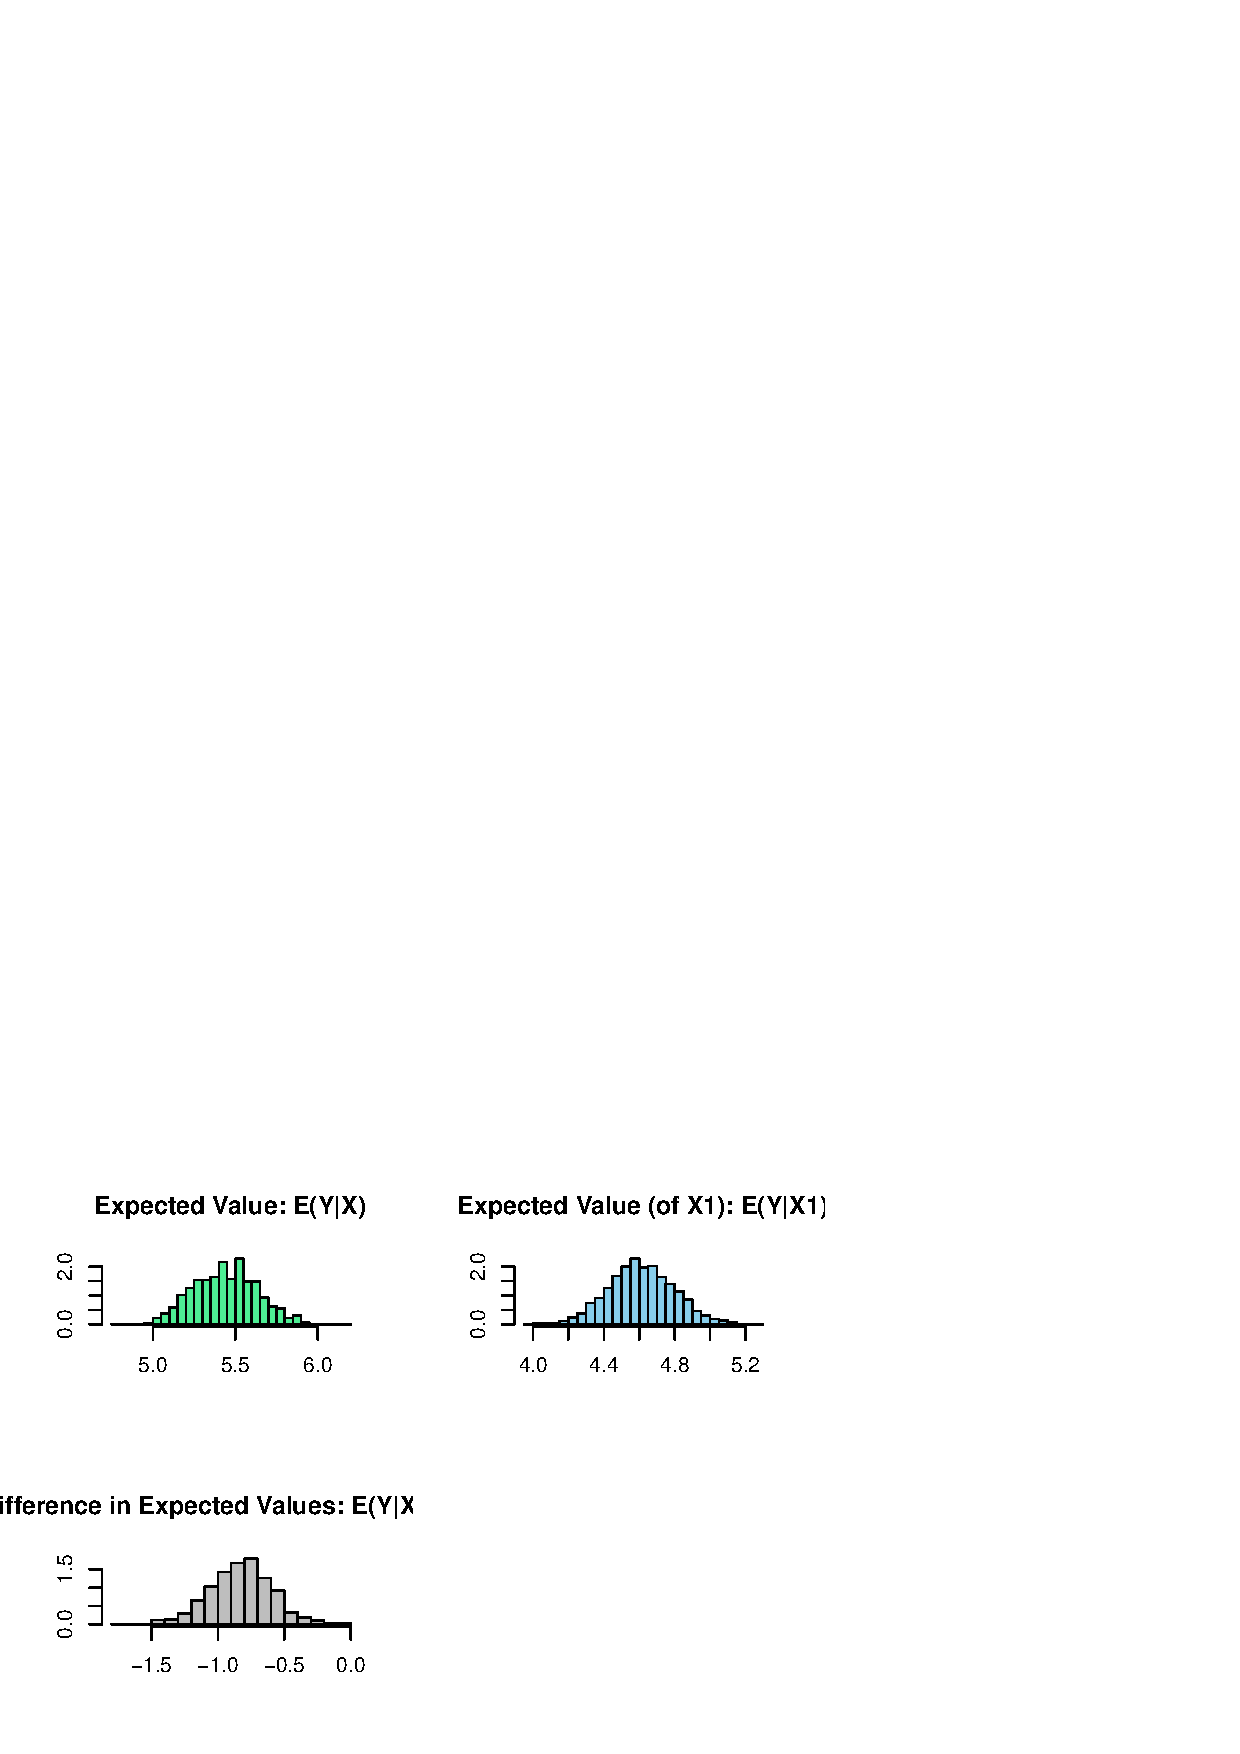
\includegraphics{vigpics/ls-ExamplesPlot}
\end{center}

\item Using Dummy Variables

Estimate a model with fixed effects for each country (see
\Sref{factors} for help with dummy variables).  Note that you do not
need to create dummy variables, as the program will automatically
parse the unique values in the selected variable into discrete levels.  
\begin{Schunk}
\begin{Sinput}
> z.out2 <- zelig(unem ~ gdp + trade + capmob + as.factor(country), 
+     model = "ls", data = macro)
\end{Sinput}
\end{Schunk}
Set values for the explanatory variables, using the default mean/mode
values, with country set to the United States and Japan, respectively:
\begin{Schunk}
\begin{Sinput}
> x.US <- setx(z.out2, country = "United States")
> x.Japan <- setx(z.out2, country = "Japan")
\end{Sinput}
\end{Schunk}
Simulate quantities of interest:
\begin{Schunk}
\begin{Sinput}
> s.out2 <- sim(z.out2, x = x.US, x1 = x.Japan)
\end{Sinput}
\end{Schunk}
\begin{center}
\begin{Schunk}
\begin{Sinput}
> plot(s.out2)
\end{Sinput}
\end{Schunk}
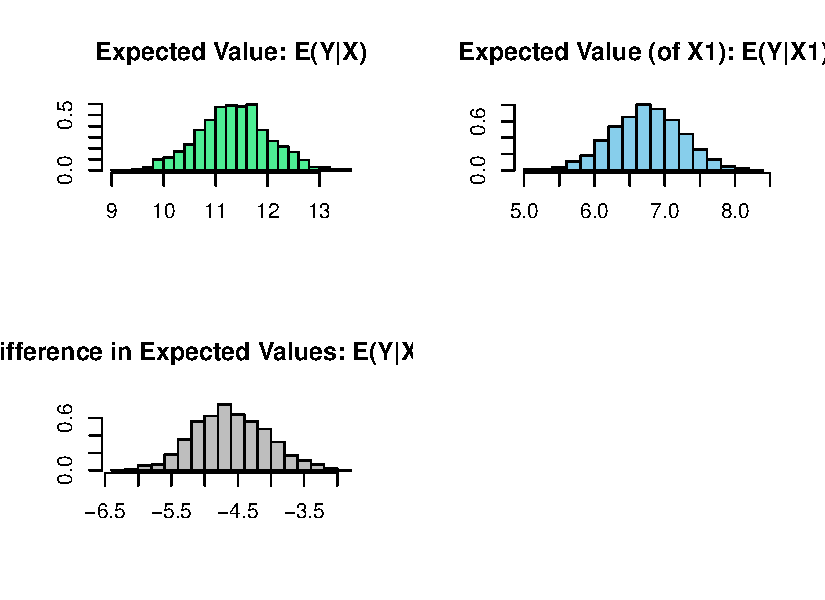
\includegraphics{vigpics/ls-DummyPlot}
\end{center}

% \item Multiple responses (least squares regression will be fitted
%   separately to each dependent variable)

% Two responses for data set macro: 
% <<Multiple.zelig>>=
%  z.out3 <- zelig(cbind(unem, gdp) ~ capmob + trade,model = "ls", data = macro)
% @
% <<Multiple.zelig.summary>>=
% summary(z.out3)
% @    
% Set values for the explanatory variables, using the default mean/mode
% values, with country set to the United States and Japan, respectively:
% <<Multiple.setx>>=
%  x.US <- setx(z.out3, country = "United States")
%  x.Japan <- setx(z.out3, country = "Japan")
% @ 
% Simulate quantities of interest:
% <<Multiple.sim>>=
%  s.out3 <- sim(z.out3, x = x.US, x1 = x.Japan)
% @
% Summary
% <<Example4.sim.summary>>=
% summary(s.out3)
% @  
% \begin{center}
% <<label=Example4Plot,fig=true,echo=true,  width=7.5, height=6>>= 
%  plot(s.out3)
% @ 
%\end{center}

\end{enumerate}

\subsubsection{Model}
\begin{itemize}
\item The \emph{stochastic component} is described by a density
  with mean $\mu_i$ and the common variance $\sigma^2$
  \begin{equation*}
    Y_i \; \sim \; f(y_i \mid \mu_i, \sigma^2).
  \end{equation*}
\item The \emph{systematic component} models the conditional mean as
  \begin{equation*}
     \mu_i =  x_i \beta
  \end{equation*} 
  where $x_i$ is the vector of covariates, and $\beta$ is the vector
  of coefficients.
  
  The least squares estimator is the best linear predictor of a
  dependent variable given $x_i$, and minimizes the sum of squared
  residuals, $\sum_{i=1}^n (Y_i-x_i \beta)^2$.  
\end{itemize}

\subsubsection{Quantities of Interest} 
\begin{itemize}
\item The expected value ({\tt qi\$ev}) is the mean of simulations
  from the stochastic component,  
\begin{equation*}
E(Y) = x_i \beta,\end{equation*}
given a draw of $\beta$ from its sampling distribution.  

\item In conditional prediction models, the average expected treatment
  effect ({\tt att.ev}) for the treatment group is 
    \begin{equation*} \frac{1}{\sum_{i=1}^n t_i}\sum_{i:t_i=1}^n \left\{ Y_i(t_i=1) -
      E[Y_i(t_i=0)] \right\},
    \end{equation*} 
    where $t_i$ is a binary explanatory variable defining the treatment
    ($t_i=1$) and control ($t_i=0$) groups.  Variation in the
    simulations are due to uncertainty in simulating $E[Y_i(t_i=0)]$,
    the counterfactual expected value of $Y_i$ for observations in the
    treatment group, under the assumption that everything stays the
    same except that the treatment indicator is switched to $t_i=0$.

\end{itemize}

\subsubsection{Output Values}

The output of each Zelig command contains useful information which you
may view.  For example, if you run \texttt{z.out <- zelig(y \~\,
  x, model = "ls", data)}, then you may examine the available
information in \texttt{z.out} by using \texttt{names(z.out)},
see the {\tt coefficients} by using {\tt z.out\$coefficients}, and
a default summary of information through \texttt{summary(z.out)}.
Other elements available through the {\tt \$} operator are listed
below.

\begin{itemize}
  \item From the {\tt zelig()} output object {\tt z.out}, you may
  extract:
   \begin{itemize}
   \item {\tt coefficients}: parameter estimates for the explanatory
     variables.
   \item {\tt residuals}: the working residuals in the final iteration
     of the IWLS fit.
   \item {\tt fitted.values}: fitted values.
   \item {\tt df.residual}: the residual degrees of freedom.
   \item {\tt zelig.data}: the input data frame if {\tt save.data = TRUE}.  
   \end{itemize}
  
\item From {\tt summary(z.out)}, you may extract:
   \begin{itemize}
   \item {\tt coefficients}: the parameter estimates with their
     associated standard errors, $p$-values, and $t$-statistics.
     \begin{equation*}
       \hat{\beta} \; = \; \left(\sum_{i=1}^n x_i' x_i\right)^{-1} \sum x_i y_i
     \end{equation*}
   \item {\tt sigma}: the square root of the estimate variance of the
     random error $e$:
     \begin{equation*}
       \hat{\sigma} \; = \; \frac{\sum (Y_i-x_i\hat{\beta})^2}{n-k}
     \end{equation*}
   \item {\tt r.squared}: the fraction of the variance explained by
     the model. 
     \begin{equation*}
       R^2 \; = \; 1 - \frac{\sum (Y_i-x_i\hat{\beta})^2}{\sum (y_i -
         \bar{y})^2} 
     \end{equation*}
   \item {\tt adj.r.squared}: the above $R^2$ statistic, penalizing
     for an increased number of explanatory variables.  
   \item{\tt cov.unscaled}: a $k \times k$ matrix of unscaled
     covariances.  
   \end{itemize}
   
\item From the {\tt sim()} output object {\tt s.out}, you may extract
  quantities of interest arranged as matrices indexed by simulation
  $\times$ {\tt x}-observation (for more than one {\tt x}-observation).
  Available quantities are:

   \begin{itemize}
   \item {\tt qi\$ev}: the simulated expected values for the specified
     values of {\tt x}.
   \item {\tt qi\$fd}:  the simulated first differences (or
     differences in expected values) for the specified values of {\tt
       x} and {\tt x1}. 
   \item {\tt qi\$att.ev}: the simulated average expected treatment
     effect for the treated from conditional prediction models.  
   \end{itemize}
\end{itemize}

\subsection* {How to Cite} 

\CiteZelig

\subsection* {See also}
The least squares regression is part of the stats package by William N.
Venables and Brian D. Ripley \citep{VenRip02}.In addition, advanced users may wish to refer to \texttt{help(lm)} and \texttt{help(lm.fit)}.Robust standard errors are implemented via the sandwich package by Achim Zeileis \citep{Zeileis04}.Sample data are from \cite{KinTomWit00}.

\bibliographystyle{asa}
\bibliography{gk,gkpubs}
 



\chapter{Gamma Regression for Continuous, Positive Dependent Variables}

\nobibliography*


\section{{\tt gamma}: Gamma Regression for Continuous, Positive Dependent Variables}\label{gamma}

Use the gamma regression model if you have a positive-valued dependent
variable such as the number of years a parliamentary cabinet endures,
or the seconds you can stay airborne while jumping.  The gamma
distribution assumes that all waiting times are complete by the end
of the study (censoring is not allowed).

\subsubsection{Syntax}

\begin{verbatim}
> z.out <- zelig(Y ~ X1 + X2, model = "gamma", data = mydata)
> x.out <- setx(z.out)
> s.out <- sim(z.out, x = x.out, x1 = NULL)
\end{verbatim}

\subsubsection{Additional Inputs} 

In addition to the standard inputs, {\tt zelig()} takes the following
additional options for gamma regression:  
\begin{itemize}
\item {\tt robust}: defaults to {\tt FALSE}.  If {\tt TRUE} is
selected, {\tt zelig()} computes robust standard errors via the {\tt
sandwich} package (see \cite{Zeileis04}).  The default type of robust
standard error is heteroskedastic and autocorrelation consistent (HAC),
and assumes that observations are ordered by time index.

In addition, {\tt robust} may be a list with the following options:  
\begin{itemize}
\item {\tt method}:  Choose from 
\begin{itemize}
\item {\tt "vcovHAC"}: (default if {\tt robust = TRUE}) HAC standard
errors. 
\item {\tt "kernHAC"}: HAC standard errors using the
weights given in \cite{Andrews91}. 
\item {\tt "weave"}: HAC standard errors using the
weights given in \cite{LumHea99}.  
\end{itemize}  
\item {\tt order.by}: defaults to {\tt NULL} (the observations are
chronologically ordered as in the original data).  Optionally, you may
specify a vector of weights (either as {\tt order.by = z}, where {\tt
z} exists outside the data frame; or as {\tt order.by = \~{}z}, where
{\tt z} is a variable in the data frame).  The observations are
chronologically ordered by the size of {\tt z}.
\item {\tt \dots}:  additional options passed to the functions 
specified in {\tt method}.   See the {\tt sandwich} library and
\cite{Zeileis04} for more options.   
\end{itemize}
\end{itemize}

\subsubsection{Example}

Attach the sample data: 
\begin{Schunk}
\begin{Sinput}
> data(coalition)
\end{Sinput}
\end{Schunk}
Estimate the model: 
\begin{Schunk}
\begin{Sinput}
> z.out <- zelig(duration ~ fract + numst2, model = "gamma", data = coalition)
\end{Sinput}
\end{Schunk}
View the regression output:  
\begin{Schunk}
\begin{Sinput}
> summary(z.out)
\end{Sinput}
\end{Schunk}
Set the baseline values (with the ruling coalition in the minority)
and the alternative values (with the ruling coalition in the majority)
for X:
\begin{Schunk}
\begin{Sinput}
> x.low <- setx(z.out, numst2 = 0)
> x.high <- setx(z.out, numst2 = 1)
\end{Sinput}
\end{Schunk}
Simulate expected values ({\tt qi\$ev}) and first differences ({\tt qi\$fd}):
\begin{Schunk}
\begin{Sinput}
> s.out <- sim(z.out, x = x.low, x1 = x.high)
\end{Sinput}
\end{Schunk}
\begin{Schunk}
\begin{Sinput}
> summary(s.out)
\end{Sinput}
\end{Schunk}
\begin{center}
\begin{Schunk}
\begin{Sinput}
> plot(s.out)
\end{Sinput}
\end{Schunk}
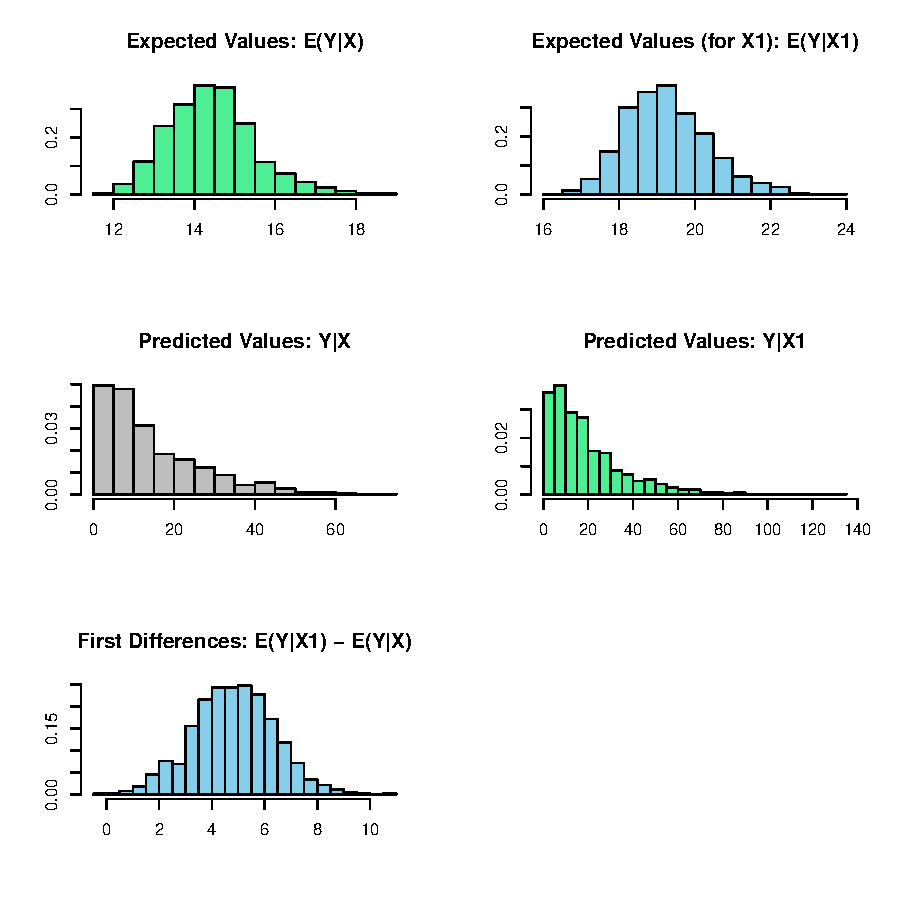
\includegraphics{vigpics/gamma-ExamplePlot}
\end{center}

\subsubsection{Model}

\begin{itemize}
\item The Gamma distribution with scale parameter $\alpha$ has a
\emph{stochastic component}:
\begin{eqnarray*}
Y &\sim& \textrm{Gamma}(y_i \mid \lambda_i, \alpha) \\
f(y)  &=& \frac{1}{\alpha^{\lambda_i} \, \Gamma \lambda_i} \, y_i^{\lambda_i
  - 1} \exp -\left\{ \frac{y_i}{\alpha} \right\}
\end{eqnarray*}
for $\alpha, \lambda_i, y_i > 0$.  \\

\item The \emph{systematic component} is given by
\begin{equation*}
  \lambda_i = \frac{1}{x_i \beta}
\end{equation*}
\end{itemize}

\subsubsection{Quantities of Interest}

\begin{itemize}
\item The expected values ({\tt qi\$ev}) are simulations of the mean
  of the stochastic component given draws of $\alpha$ and
  $\beta$ from their posteriors:  $$E(Y) = \alpha \lambda_i.$$  
\item The predicted values ({\tt qi\$pr}) are draws from the gamma
  distribution for each given set of parameters $(\alpha, \lambda_i)$.
\item If {\tt x1} is specified, {\tt sim()} also returns the
  differences in the expected values ({\tt qi\$fd}), $$E(Y \mid x_1) -
  E(Y \mid x)$$.

\item In conditional prediction models, the average expected treatment
  effect ({\tt att.ev}) for the treatment group is 
    \begin{equation*} \frac{1}{\sum_{i=1}^n t_i}\sum_{i:t_i=1}^n \left\{ Y_i(t_i=1) -
      E[Y_i(t_i=0)] \right\},
    \end{equation*} 
    where $t_i$ is a binary explanatory variable defining the treatment
    ($t_i=1$) and control ($t_i=0$) groups.  Variation in the
    simulations are due to uncertainty in simulating $E[Y_i(t_i=0)]$,
    the counterfactual expected value of $Y_i$ for observations in the
    treatment group, under the assumption that everything stays the
    same except that the treatment indicator is switched to $t_i=0$.

\item In conditional prediction models, the average predicted treatment
  effect ({\tt att.pr}) for the treatment group is 
    \begin{equation*} \frac{1}{\sum_{i=1}^n t_i}\sum_{i:t_i=1}^n \left\{ Y_i(t_i=1) -
      \widehat{Y_i(t_i=0)} \right\},
    \end{equation*} 
    where $t_i$ is a binary explanatory variable defining the treatment
    ($t_i=1$) and control ($t_i=0$) groups.  Variation in the
    simulations are due to uncertainty in simulating
    $\widehat{Y_i(t_i=0)}$, the counterfactual predicted value of
    $Y_i$ for observations in the treatment group, under the
    assumption that everything stays the same except that the
    treatment indicator is switched to $t_i=0$.  

\end{itemize}

\subsubsection{Output Values}

The output of each Zelig command contains useful information which you
may view.  For example, if you run \texttt{z.out <- zelig(y \~\,
  x, model = "gamma", data)}, then you may examine the available
information in \texttt{z.out} by using \texttt{names(z.out)},
see the {\tt coefficients} by using {\tt z.out\$coefficients}, and
a default summary of information through \texttt{summary(z.out)}.
Other elements available through the {\tt \$} operator are listed
below.

\begin{itemize}
\item From the {\tt zelig()} output object {\tt z.out}, you may
  extract:
   \begin{itemize}
   \item {\tt coefficients}: parameter estimates for the explanatory
     variables.
   \item {\tt residuals}: the working residuals in the final iteration
     of the IWLS fit.
   \item {\tt fitted.values}: the vector of fitted values.
   \item {\tt linear.predictors}: the vector of $x_{i}\beta$.
   \item {\tt aic}: Akaike's Information Criterion (minus twice the
     maximized log-likelihood plus twice the number of coefficients).
   \item {\tt df.residual}: the residual degrees of freedom.
   \item {\tt df.null}: the residual degrees of freedom for the null
     model.
   \item {\tt zelig.data}: the input data frame if {\tt save.data = TRUE}.  
   \end{itemize}

\item From {\tt summary(z.out)}, you may extract: 
   \begin{itemize}
   \item {\tt coefficients}: the parameter estimates with their
     associated standard errors, $p$-values, and $t$-statistics.
   \item{\tt cov.scaled}: a $k \times k$ matrix of scaled covariances.
   \item{\tt cov.unscaled}: a $k \times k$ matrix of unscaled
     covariances.  
   \end{itemize}

\item From the {\tt sim()} output object {\tt s.out}, you may extract
  quantities of interest arranged as matrices indexed by simulation
  $\times$ {\tt x}-observation (for more than one {\tt x}-observation).
  Available quantities are:

   \begin{itemize}
   \item {\tt qi\$ev}: the simulated expected values for the specified
     values of {\tt x}.
   \item {\tt qi\$pr}: the simulated predicted values drawn from a
     distribution defined by $(\alpha, \lambda_i)$.
   \item {\tt qi\$fd}: the simulated first difference in the expected
     values for the specified values in {\tt x} and {\tt x1}.
   \item {\tt qi\$att.ev}: the simulated average expected treatment
     effect for the treated from conditional prediction models.  
   \item {\tt qi\$att.pr}: the simulated average predicted treatment
     effect for the treated from conditional prediction models.  
   \end{itemize}
\end{itemize}


\subsection* {How to Cite} 


To cite Zelig as a whole, please reference these two sources:
\begin{verse}
  Kosuke Imai, Gary King, and Olivia Lau. 2007. ``Zelig: Everyone's
  Statistical Software,'' \url{http://GKing.harvard.edu/zelig}.
\end{verse}
\begin{verse}
Imai, Kosuke, Gary King, and Olivia Lau. (2008). ``Toward A Common Framework for Statistical Analysis and Development.'' Journal of Computational and Graphical Statistics, Vol. 17, No. 4 (December), pp. 892-913. 
\end{verse}


\subsection* {See also}
The gamma model is part of the stats package by \citet{VenRip02}.
Advanced users may wish to refer to \texttt{help(glm)} and
\texttt{help(family)}, as well as \cite{McCNel89}. Robust standard
errors are implemented via the sandwich package by \citet{Zeileis04}.
Sample data are from \cite{KinTomWit00}.

\bibliographystyle{asa}
\bibliography{gk,gkpubs}
 



\chapter{Poisson Regression for Event Count Dependent Variables}

\nobibliography*


\section{{\tt poisson}: Poisson Regression for Event Count
Dependent Variables}\label{poisson}

Use the Poisson regression model if the observations of your dependent
variable represents the number of independent events that occur during
a fixed period of time (see the negative binomial model, \Sref{negbin},
for over-dispersed event counts.)  For a Bayesian implementation of
this model, see \Sref{poisson.bayes}.  

\subsubsection{Syntax}

\begin{verbatim}
> z.out <- zelig(Y ~ X1 + X2, model = "poisson", data = mydata)
> x.out <- setx(z.out)
> s.out <- sim(z.out, x = x.out)
\end{verbatim}

\subsubsection{Additional Inputs} 

In addition to the standard inputs, {\tt zelig()} takes the following
additional options for poisson regression:  
\begin{itemize}
\item {\tt robust}: defaults to {\tt FALSE}.  If {\tt TRUE} is
selected, {\tt zelig()} computes robust standard errors via the {\tt
sandwich} package (see \cite{Zeileis04}).  The default type of robust
standard error is heteroskedastic and autocorrelation consistent (HAC),
and assumes that observations are ordered by time index.

In addition, {\tt robust} may be a list with the following options:  
\begin{itemize}
\item {\tt method}:  Choose from 
\begin{itemize}
\item {\tt "vcovHAC"}: (default if {\tt robust = TRUE}) HAC standard
errors. 
\item {\tt "kernHAC"}: HAC standard errors using the
weights given in \cite{Andrews91}. 
\item {\tt "weave"}: HAC standard errors using the
weights given in \cite{LumHea99}.  
\end{itemize}  
\item {\tt order.by}: defaults to {\tt NULL} (the observations are
chronologically ordered as in the original data).  Optionally, you may
specify a vector of weights (either as {\tt order.by = z}, where {\tt
z} exists outside the data frame; or as {\tt order.by = \~{}z}, where
{\tt z} is a variable in the data frame).  The observations are
chronologically ordered by the size of {\tt z}.
\item {\tt \dots}:  additional options passed to the functions 
specified in {\tt method}.   See the {\tt sandwich} library and
\cite{Zeileis04} for more options.   
\end{itemize}
\end{itemize}

\subsubsection{Example}

Load sample data:  
\begin{Schunk}
\begin{Sinput}
> data(sanction)
\end{Sinput}
\end{Schunk}
Estimate Poisson model:  
\begin{Schunk}
\begin{Sinput}
> z.out <- zelig(num ~ target + coop, model = "poisson", data = sanction)
\end{Sinput}
\end{Schunk}
\begin{Schunk}
\begin{Sinput}
> summary(z.out)
\end{Sinput}
\end{Schunk}
Set values for the explanatory variables to their default mean values:  
\begin{Schunk}
\begin{Sinput}
> x.out <- setx(z.out)
\end{Sinput}
\end{Schunk}
Simulate fitted values:  
\begin{Schunk}
\begin{Sinput}
> s.out <- sim(z.out, x = x.out)
\end{Sinput}
\end{Schunk}
\begin{Schunk}
\begin{Sinput}
> summary(s.out)
\end{Sinput}
\end{Schunk}
\begin{center}
\begin{Schunk}
\begin{Sinput}
> plot(s.out)
\end{Sinput}
\end{Schunk}
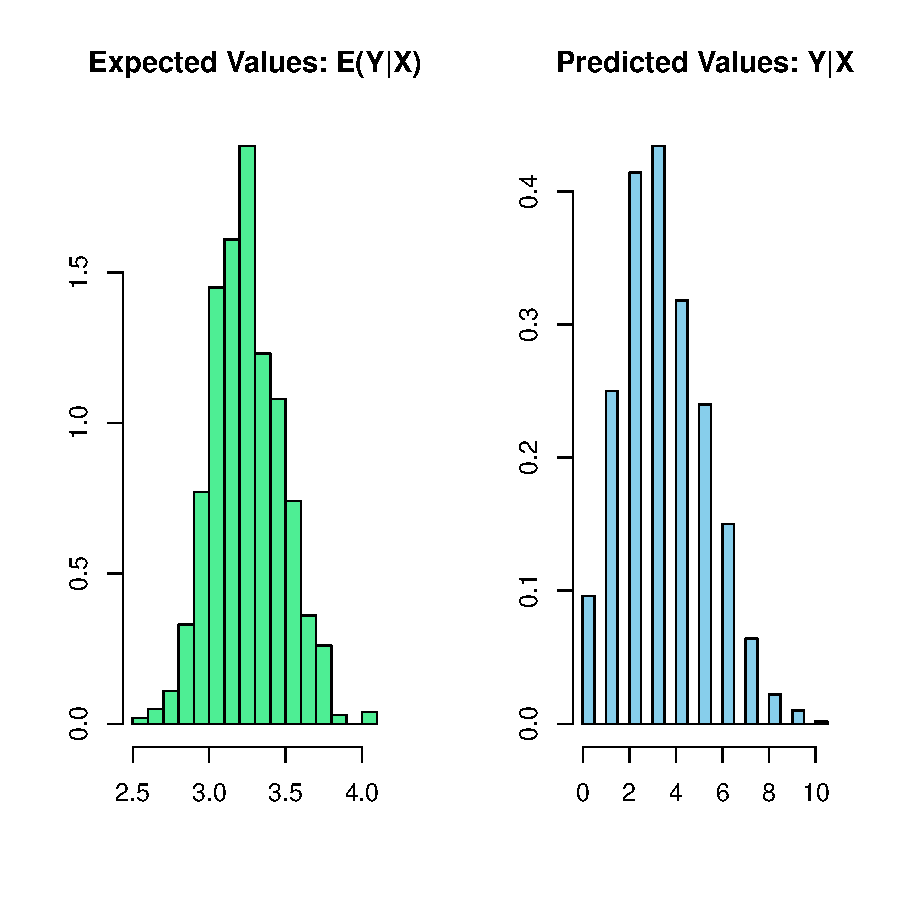
\includegraphics{vigpics/poisson-ExamplePlot}
\end{center}

\subsubsection{Model}
Let $Y_i$ be the number of independent events that occur during a
fixed time period. This variable can take any non-negative integer.

\begin{itemize}
\item The Poisson distribution has \emph{stochastic component}
  \begin{equation*}
    Y_i \; \sim \; \textrm{Poisson}(\lambda_i),
  \end{equation*}
  where $\lambda_i$ is the mean and variance parameter.
  
\item The \emph{systematic component} is 
  \begin{equation*}
    \lambda_i \; = \; \exp(x_i \beta),
  \end{equation*}
  where $x_i$ is the vector of explanatory variables, and $\beta$ is
  the vector of coefficients.
\end{itemize}

\subsubsection{Quantities of Interest}

\begin{itemize}
  
\item The expected value ({\tt qi\$ev}) is the mean of simulations
  from the stochastic component, $$E(Y) = \lambda_i =  \exp(x_i
  \beta),$$ given draws of $\beta$ from its sampling distribution.  
  
\item The predicted value ({\tt qi\$pr}) is a random draw from the
  poisson distribution defined by mean $\lambda_i$.

\item The first difference in the expected values ({\tt qi\$fd}) is given by:
\begin{equation*}
\textrm{FD} \; = \; E(Y | x_1) - E(Y \mid x)
\end{equation*}
\item In conditional prediction models, the average expected treatment
  effect ({\tt att.ev}) for the treatment group is 
    \begin{equation*} \frac{1}{\sum_{i=1}^n t_i}\sum_{i:t_i=1}^n \left\{ Y_i(t_i=1) -
      E[Y_i(t_i=0)] \right\},
    \end{equation*} 
    where $t_i$ is a binary explanatory variable defining the treatment
    ($t_i=1$) and control ($t_i=0$) groups.  Variation in the
    simulations are due to uncertainty in simulating $E[Y_i(t_i=0)]$,
    the counterfactual expected value of $Y_i$ for observations in the
    treatment group, under the assumption that everything stays the
    same except that the treatment indicator is switched to $t_i=0$.

\item In conditional prediction models, the average predicted treatment
  effect ({\tt att.pr}) for the treatment group is 
    \begin{equation*} \frac{1}{\sum_{i=1}^n t_i}\sum_{i:t_i=1}^n \left\{ Y_i(t_i=1) -
      \widehat{Y_i(t_i=0)} \right\},
    \end{equation*} 
    where $t_i$ is a binary explanatory variable defining the
    treatment ($t_i=1$) and control ($t_i=0$) groups.  Variation in
    the simulations are due to uncertainty in simulating
    $\widehat{Y_i(t_i=0)}$, the counterfactual predicted value of
    $Y_i$ for observations in the treatment group, under the
    assumption that everything stays the same except that the
    treatment indicator is switched to $t_i=0$.
\end{itemize}

\subsubsection{Output Values}

The output of each Zelig command contains useful information which you
may view.  For example, if you run \texttt{z.out <- zelig(y \~\,
  x, model = "poisson", data)}, then you may examine the available
information in \texttt{z.out} by using \texttt{names(z.out)},
see the {\tt coefficients} by using {\tt z.out\$coefficients}, and
a default summary of information through \texttt{summary(z.out)}.
Other elements available through the {\tt \$} operator are listed
below.

\begin{itemize}
\item From the {\tt zelig()} output object {\tt z.out}, you may extract:
   \begin{itemize}
   \item {\tt coefficients}: parameter estimates for the explanatory
     variables.
   \item {\tt residuals}: the working residuals in the final iteration
     of the IWLS fit.
   \item {\tt fitted.values}: a vector of the fitted values for the systemic
     component $\lambda$.  
   \item {\tt linear.predictors}: a vector of $x_{i}\beta$.  
   \item {\tt aic}: Akaike's Information Criterion (minus twice the
     maximized log-likelihood plus twice the number of coefficients).
   \item {\tt df.residual}: the residual degrees of freedom.
   \item {\tt df.null}: the residual degrees of freedom for the null
     model.
   \item {\tt zelig.data}: the input data frame if {\tt save.data = TRUE}.  
   \end{itemize}

\item From {\tt summary(z.out)}, you may extract: 
   \begin{itemize}
   \item {\tt coefficients}: the parameter estimates with their
     associated standard errors, $p$-values, and $t$-statistics.
   \item{\tt cov.scaled}: a $k \times k$ matrix of scaled covariances.
   \item{\tt cov.unscaled}: a $k \times k$ matrix of unscaled
     covariances.  
   \end{itemize}

\item From the {\tt sim()} output object {\tt s.out}, you may extract
  quantities of interest arranged as matrices indexed by simulation
  $\times$ {\tt x}-observation (for more than one {\tt x}-observation).
  Available quantities are:

   \begin{itemize}
   \item {\tt qi\$ev}: the simulated expected values given the
     specified values of {\tt x}.
   \item {\tt qi\$pr}: the simulated predicted values drawn from the
     distributions defined by $\lambda_i$.
   \item {\tt qi\$fd}: the simulated first differences in the expected
     values given the specified values of {\tt x} and {\tt x1}.
   \item {\tt qi\$att.ev}: the simulated average expected treatment
     effect for the treated from conditional prediction models.  
   \item {\tt qi\$att.pr}: the simulated average predicted treatment
     effect for the treated from conditional prediction models.  
   \end{itemize}
\end{itemize}

\subsection* {How to Cite} 

How to cite this model in Zelig:
\begin{verse}
  Kosuke Imai, Gary King, and Olivia Lau. 2007. "poisson: Poisson Regression for Event Count Dependent Variables" in Kosuke Imai, Gary King, and Olivia Lau, "Zelig: Everyone's Statistical Software,"http://gking.harvard.edu/zelig
\end{verse}
\CiteZelig
\subsection* {See also}
The poisson model is part of the stats package by \citet{VenRip02}.
Advanced users may wish to refer to \texttt{help(glm)} and
\texttt{help(family)}, as well as \cite{McCNel89}. Robust standard
errors are implemented via the sandwich package by \citet{Zeileis04}.
Sample data are from \cite{Martin92}.

\bibliographystyle{asa}
\bibliography{gk,gkpubs}
 



\chapter{Logistic Regression for Dichotomous Dependent Variables}

\nobibliography*


\section{{\tt logit}: Logistic Regression for Dichotomous Dependent
Variables}\label{logit}

Logistic regression specifies a dichotomous dependent variable as a
function of a set of explanatory variables.  For a Bayesian
implementation, see \Sref{logit.bayes}.  

\subsubsection{Syntax}

\begin{verbatim}
> z.out <- zelig(Y ~ X1 + X2, model = "logit", data = mydata)
> x.out <- setx(z.out)
> s.out <- sim(z.out, x = x.out, x1 = NULL)
\end{verbatim}

\subsubsection{Additional Inputs} 

In addition to the standard inputs, {\tt zelig()} takes the following
additional options for logistic regression:  
\begin{itemize}
\item {\tt robust}: defaults to {\tt FALSE}.  If {\tt TRUE} is
selected, {\tt zelig()} computes robust standard errors via the {\tt
sandwich} package (see \cite{Zeileis04}).  The default type of robust
standard error is heteroskedastic and autocorrelation consistent (HAC),
and assumes that observations are ordered by time index.

In addition, {\tt robust} may be a list with the following options:  
\begin{itemize}
\item {\tt method}:  Choose from 
\begin{itemize}
\item {\tt "vcovHAC"}: (default if {\tt robust = TRUE}) HAC standard
errors. 
\item {\tt "kernHAC"}: HAC standard errors using the
weights given in \cite{Andrews91}. 
\item {\tt "weave"}: HAC standard errors using the
weights given in \cite{LumHea99}.  
\end{itemize}  
\item {\tt order.by}: defaults to {\tt NULL} (the observations are
chronologically ordered as in the original data).  Optionally, you may
specify a vector of weights (either as {\tt order.by = z}, where {\tt
z} exists outside the data frame; or as {\tt order.by = \~{}z}, where
{\tt z} is a variable in the data frame)  The observations are
chronologically ordered by the size of {\tt z}.
\item {\tt \dots}:  additional options passed to the functions 
specified in {\tt method}.   See the {\tt sandwich} library and
\cite{Zeileis04} for more options.   
\end{itemize}
\end{itemize}

\subsubsection{Examples}
\begin{enumerate}
\item {Basic Example}
 
Attaching the sample turnout dataset:
\begin{Schunk}
\begin{Sinput}
> data(turnout)
\end{Sinput}
\end{Schunk}
Estimating parameter values for the logistic regression:
\begin{Schunk}
\begin{Sinput}
> z.out1 <- zelig(vote ~ age + race, model = "logit", data = turnout)
\end{Sinput}
\end{Schunk}
Setting values for the explanatory variables:
\begin{Schunk}
\begin{Sinput}
> x.out1 <- setx(z.out1, age = 36, race = "white")
\end{Sinput}
\end{Schunk}
Simulating quantities of interest from the posterior distribution.
\begin{Schunk}
\begin{Sinput}
> s.out1 <- sim(z.out1, x = x.out1)
\end{Sinput}
\end{Schunk}
\begin{Schunk}
\begin{Sinput}
> summary(s.out1)
\end{Sinput}
\end{Schunk}
\begin{center}
\begin{Schunk}
\begin{Sinput}
> plot(s.out1)
\end{Sinput}
\end{Schunk}
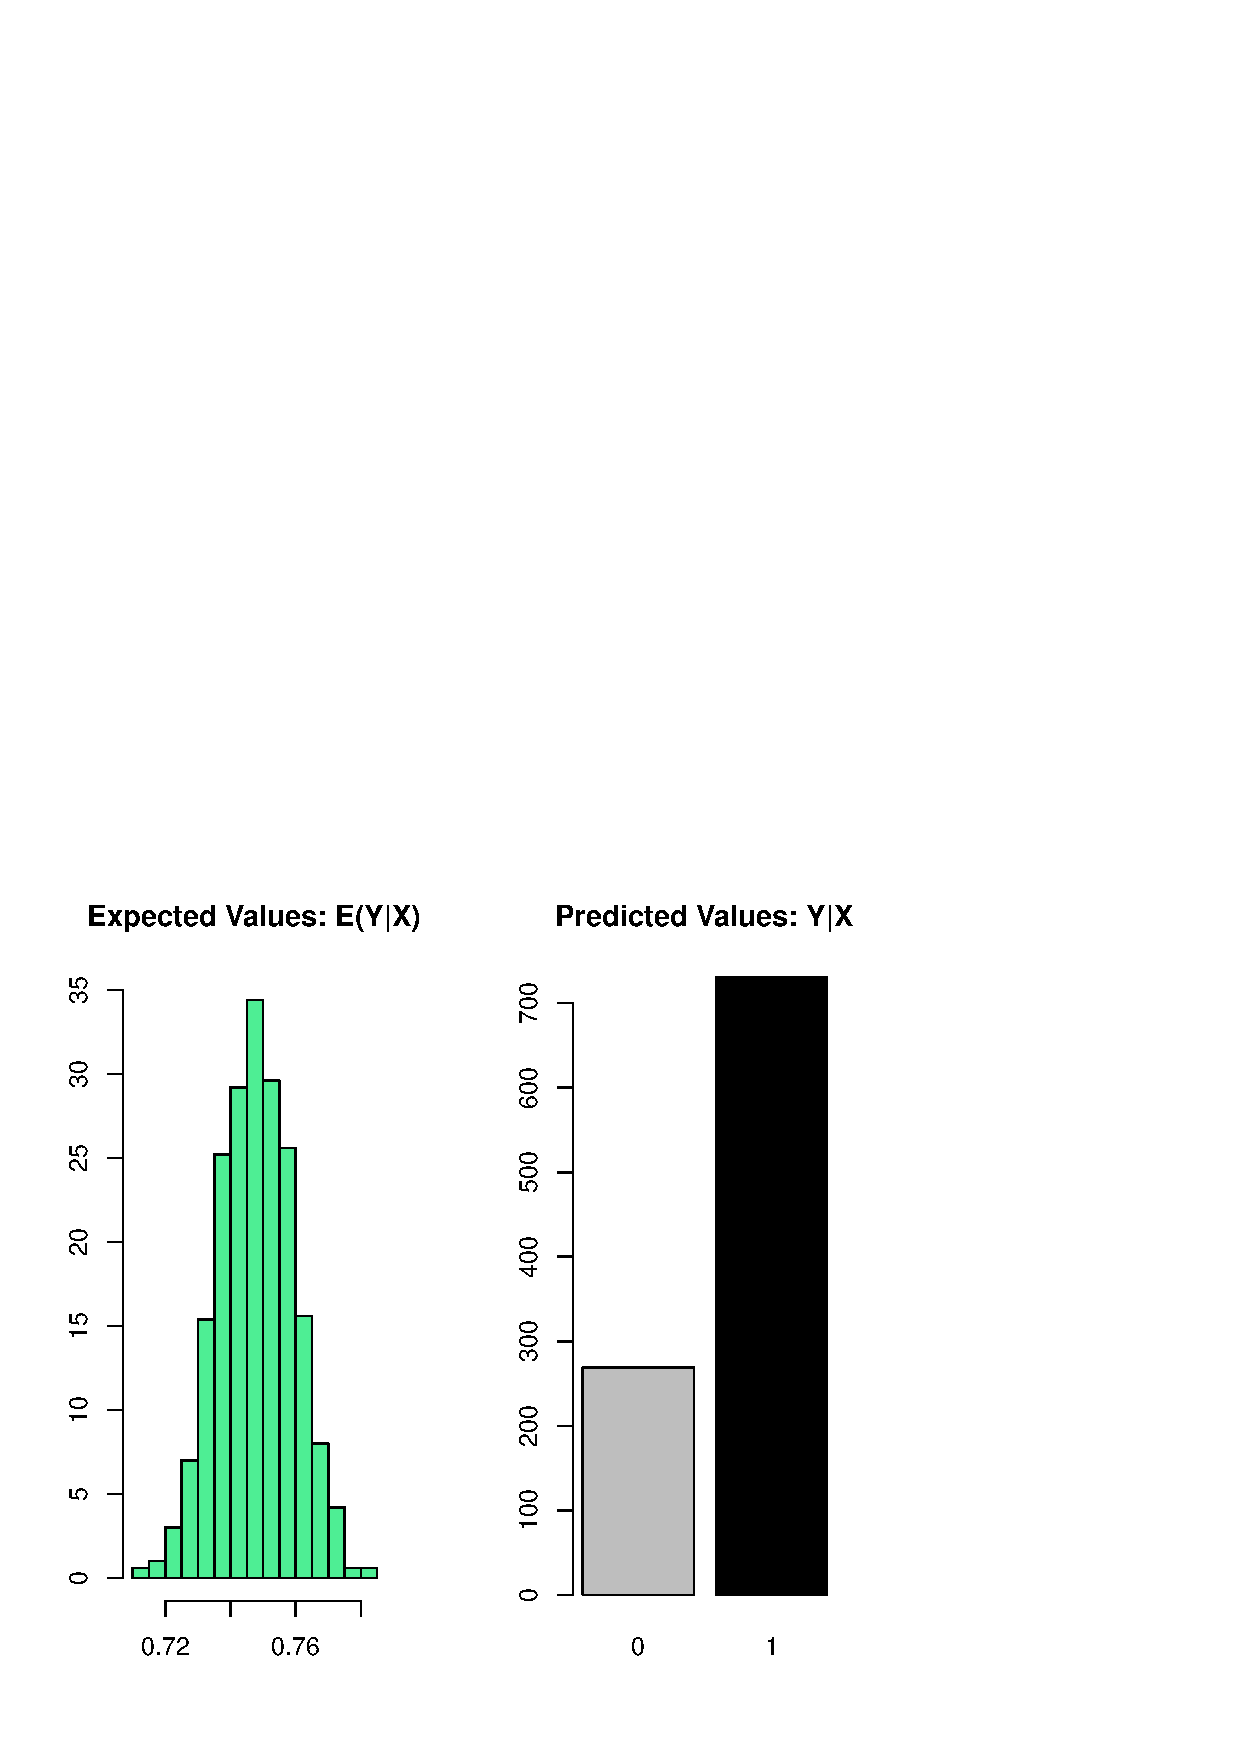
\includegraphics{vigpics/logit-ExamplePlot}
\end{center}

\item {Simulating First Differences}

Estimating the risk difference (and risk ratio) between low education
(25th percentile) and high education (75th percentile) while all the
other variables held at their default values.
\begin{Schunk}
\begin{Sinput}
> z.out2 <- zelig(vote ~ race + educate, model = "logit", data = turnout)
> x.high <- setx(z.out2, educate = quantile(turnout$educate, prob = 0.75))
> x.low <- setx(z.out2, educate = quantile(turnout$educate, prob = 0.25))
\end{Sinput}
\end{Schunk}

\begin{Schunk}
\begin{Sinput}
> s.out2 <- sim(z.out2, x = x.high, x1 = x.low)
\end{Sinput}
\end{Schunk}
\begin{Schunk}
\begin{Sinput}
> summary(s.out2)
\end{Sinput}
\end{Schunk}
\begin{center}
\begin{Schunk}
\begin{Sinput}
> plot(s.out2)
\end{Sinput}
\end{Schunk}
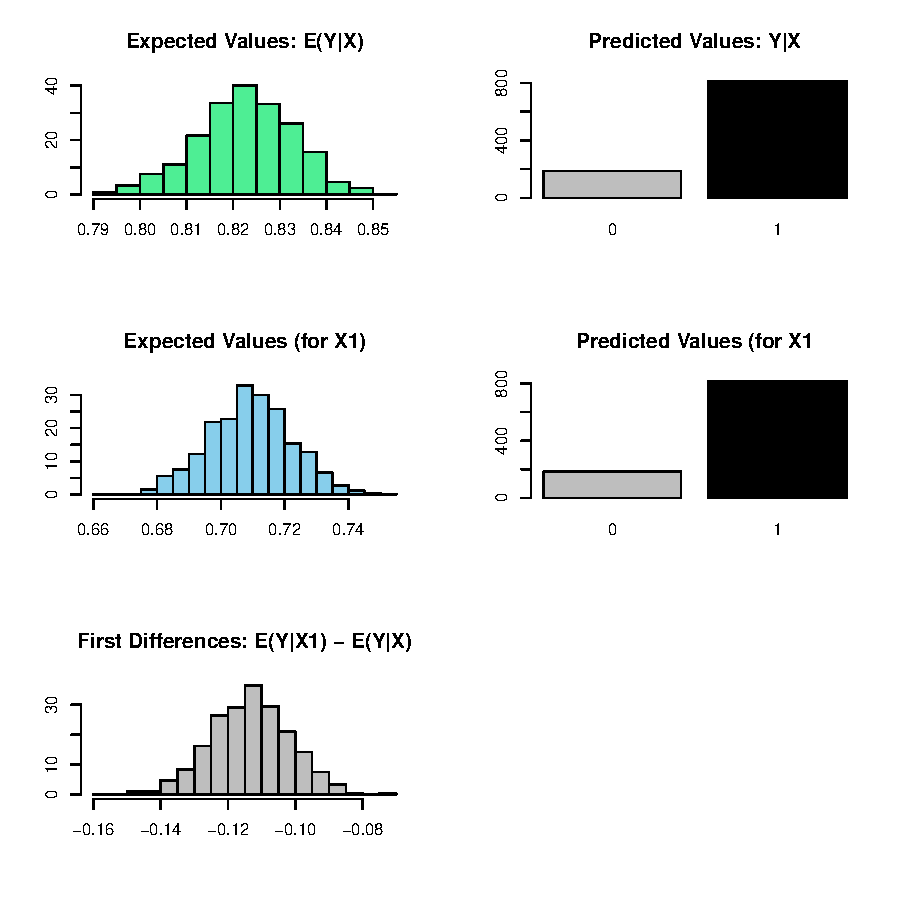
\includegraphics{vigpics/logit-FirstDifferencesPlot}
\end{center} 


\item {Presenting Results: An ROC Plot}  \label{ROC}
  
  One can use an ROC plot to evaluate the fit of alternative model
  specifications.  (Use {\tt demo(roc)} to view this example, or see
  King and Zeng (2002)\nocite{KinZen02}.)  
\begin{Schunk}
\begin{Sinput}
> z.out1 <- zelig(vote ~ race + educate + age, model = "logit", 
+     data = turnout)
> z.out2 <- zelig(vote ~ race + educate, model = "logit", data = turnout)
\end{Sinput}
\end{Schunk}
\begin{center}
\begin{Schunk}
\begin{Sinput}
> rocplot(z.out1$y, z.out2$y, fitted(z.out1), fitted(z.out2))
\end{Sinput}
\end{Schunk}
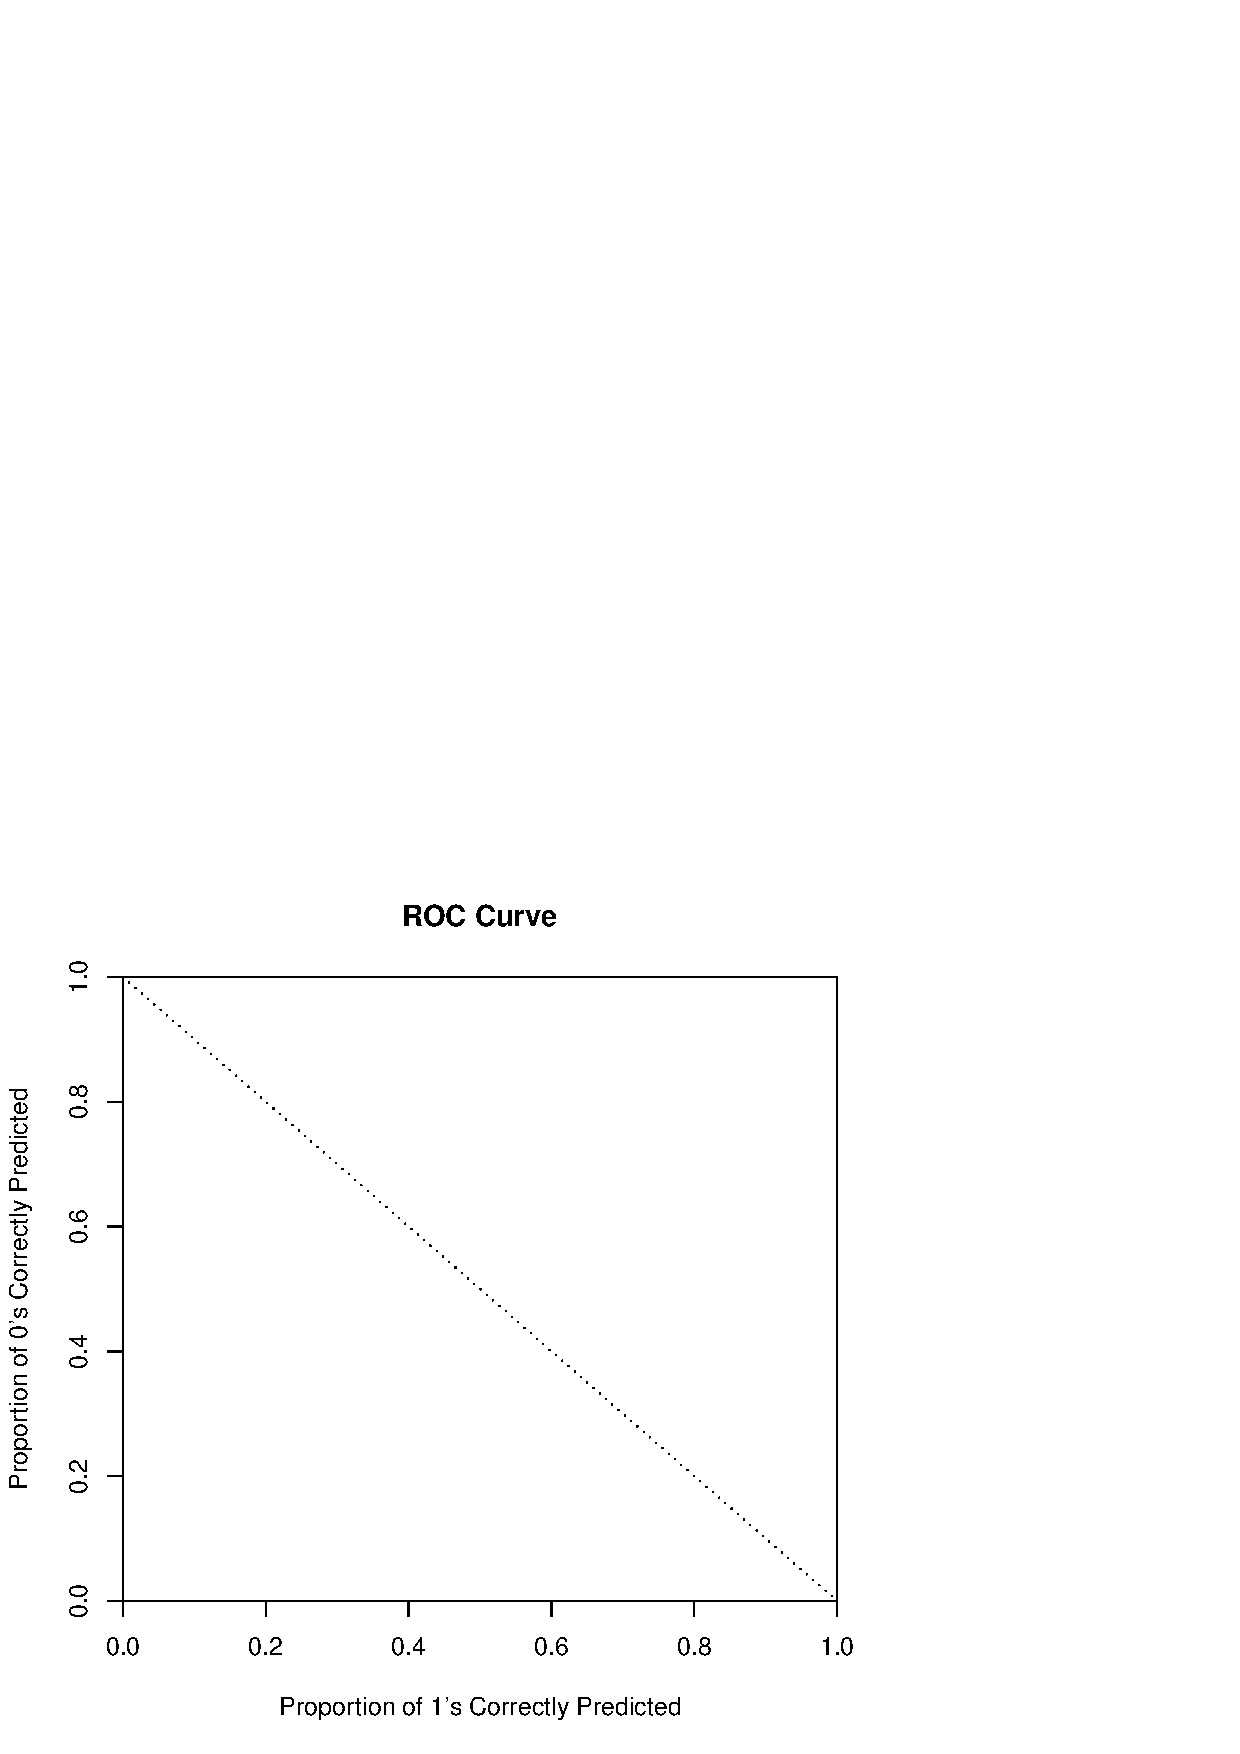
\includegraphics{vigpics/logit-ROCPlot}
\end{center}
\end{enumerate}

\subsubsection{Model}
Let $Y_i$ be the binary dependent variable for observation $i$ which
takes the value of either 0 or 1.
\begin{itemize}

\item The \emph{stochastic component} is given by  
\begin{eqnarray*}
Y_i &\sim& \textrm{Bernoulli}(y_i \mid \pi_i) \\
    &=& \pi_i^{y_i} (1-\pi_i)^{1-y_i}
\end{eqnarray*}
where $\pi_i=\Pr(Y_i=1)$.

\item The \emph{systematic component} is given by: 
\begin{equation*}
\pi_i \; = \; \frac{1}{1 + \exp(-x_i \beta)}.
\end{equation*}
where $x_i$ is the vector of $k$ explanatory variables for observation $i$
and $\beta$ is the vector of coefficients.
\end{itemize}

\subsubsection{Quantities of Interest}
\begin{itemize}
\item The expected values ({\tt qi\$ev}) for the logit model are
  simulations of the predicted probability of a success: $$E(Y) =
  \pi_i= \frac{1}{1 + \exp(-x_i \beta)},$$ given draws of $\beta$ from
  its sampling distribution.

\item The predicted values ({\tt qi\$pr}) are draws from the Binomial
  distribution with mean equal to the simulated expected value $\pi_i$.  

\item The first difference ({\tt qi\$fd}) for the logit model is defined as
\begin{equation*}
\textrm{FD} = \Pr(Y = 1 \mid x_1) - \Pr(Y = 1 \mid x).
\end{equation*}

\item The risk ratio ({\tt qi\$rr}) is defined as
\begin{equation*}
\textrm{RR} = \Pr(Y = 1 \mid x_1) \ / \ \Pr(Y = 1 \mid x).
\end{equation*}

\item In conditional prediction models, the average expected treatment
  effect ({\tt att.ev}) for the treatment group is 
    \begin{equation*} \frac{1}{\sum_{i=1}^n t_i}\sum_{i:t_i=1}^n \left\{ Y_i(t_i=1) -
      E[Y_i(t_i=0)] \right\},
    \end{equation*} 
    where $t_i$ is a binary explanatory variable defining the treatment
    ($t_i=1$) and control ($t_i=0$) groups.  Variation in the
    simulations are due to uncertainty in simulating $E[Y_i(t_i=0)]$,
    the counterfactual expected value of $Y_i$ for observations in the
    treatment group, under the assumption that everything stays the
    same except that the treatment indicator is switched to $t_i=0$.

\item In conditional prediction models, the average predicted treatment
  effect ({\tt att.pr}) for the treatment group is 
    \begin{equation*} \frac{1}{\sum_{i=1}^n t_i}\sum_{i:t_i=1}^n \left\{ Y_i(t_i=1) -
      \widehat{Y_i(t_i=0)}\right\},
    \end{equation*} 
    where $t_i$ is a binary explanatory variable defining the
    treatment ($t_i=1$) and control ($t_i=0$) groups.  Variation in
    the simulations are due to uncertainty in simulating
    $\widehat{Y_i(t_i=0)}$, the counterfactual predicted value of
    $Y_i$ for observations in the treatment group, under the
    assumption that everything stays the same except that the
    treatment indicator is switched to $t_i=0$.
\end{itemize}

\subsubsection{Output Values}

The output of each Zelig command contains useful information which you
may view.  For example, if you run \texttt{z.out <- zelig(y \~\, x,
  model = "logit", data)}, then you may examine the available
information in \texttt{z.out} by using \texttt{names(z.out)},
see the {\tt coefficients} by using {\tt z.out\$coefficients}, and
a default summary of information through \texttt{summary(z.out)}.
Other elements available through the {\tt \$} operator are listed
below.

\begin{itemize}
\item From the {\tt zelig()} output object {\tt z.out}, you may
  extract:
   \begin{itemize}
   \item {\tt coefficients}: parameter estimates for the explanatory
     variables.
   \item {\tt residuals}: the working residuals in the final iteration
     of the IWLS fit.
   \item {\tt fitted.values}: the vector of fitted values for the
     systemic component, $\pi_i$.
   \item {\tt linear.predictors}: the vector of $x_{i}\beta$
   \item {\tt aic}: Akaike's Information Criterion (minus twice the
     maximized log-likelihood plus twice the number of coefficients).
   \item {\tt df.residual}: the residual degrees of freedom.
   \item {\tt df.null}: the residual degrees of freedom for the null
     model.
   \item {\tt data}: the name of the input data frame.  
   \end{itemize}

\item From {\tt summary(z.out)}, you may extract: 
   \begin{itemize}
   \item {\tt coefficients}: the parameter estimates with their
     associated standard errors, $p$-values, and $t$-statistics.
   \item{\tt cov.scaled}: a $k \times k$ matrix of scaled covariances.
   \item{\tt cov.unscaled}: a $k \times k$ matrix of unscaled
     covariances.  
   \end{itemize}

\item From the {\tt sim()} output object {\tt s.out}, you may extract
  quantities of interest arranged as matrices indexed by simulation
  $\times$ {\tt x}-observation (for more than one {\tt x}-observation).
  Available quantities are:

   \begin{itemize}
   \item {\tt qi\$ev}: the simulated expected probabilities for the
     specified values of {\tt x}.
   \item {\tt qi\$pr}: the simulated predicted values for the
     specified values of {\tt x}.
   \item {\tt qi\$fd}: the simulated first difference in the expected
     probabilities for the values specified in {\tt x} and {\tt x1}.
   \item {\tt qi\$rr}: the simulated risk ratio for the expected
     probabilities simulated from {\tt x} and {\tt x1}.
   \item {\tt qi\$att.ev}: the simulated average expected treatment
     effect for the treated from conditional prediction models.  
   \item {\tt qi\$att.pr}: the simulated average predicted treatment
     effect for the treated from conditional prediction models.  
   \end{itemize}
\end{itemize}

\subsection* {How to Cite} 

How to cite this model in Zelig:
\begin{verse}
  Kosuke Imai, Gary King, and Olivia Lau. 2008. "logit: Logistic Regression for Dichotomous Dependent Variables" in Kosuke Imai, Gary King, and Olivia Lau, "Zelig: Everyone's Statistical Software,"http://gking.harvard.edu/zelig
\end{verse}


\CiteZelig

\subsection*{See also}

The logit model is part of the stats package by \citet{VenRip02}.
Advanced users may wish to refer to \texttt{help(glm)} and
\texttt{help(family)}, as well as \cite{McCNel89}. Robust standard
errors are implemented via the sandwich package by \citet{Zeileis04}.
Sample data are from \cite{KinTomWit00}.

\bibliographystyle{asa}
\bibliography{gk,gkpubs}
 



\chapter{Probit Regression for Dichotomous Dependent Variables}

\nobibliography*


\section{{\tt probit}: Probit Regression for Dichotomous Dependent Variables}\label{probit}

Use probit regression to model binary dependent variables
specified as a function of a set of explanatory variables.  For a
Bayesian implementation of this model, see \Sref{probit.bayes}.  

\subsubsection{Syntax}
\begin{verbatim}
> z.out <- zelig(Y ~ X1 + X2, model = "probit", data = mydata)
> x.out <- setx(z.out)
> s.out <- sim(z.out, x = x.out, x1 = NULL)
\end{verbatim}

\subsubsection{Additional Inputs} 

In addition to the standard inputs, {\tt zelig()} takes the following
additional options for probit regression:  
\begin{itemize}
\item {\tt robust}: defaults to {\tt FALSE}.  If {\tt TRUE} is
selected, {\tt zelig()} computes robust standard errors via the {\tt
sandwich} package (see \cite{Zeileis04}).  The default type of robust
standard error is heteroskedastic and autocorrelation consistent (HAC),
and assumes that observations are ordered by time index.

In addition, {\tt robust} may be a list with the following options:  
\begin{itemize}
\item {\tt method}:  Choose from 
\begin{itemize}
\item {\tt "vcovHAC"}: (default if {\tt robust = TRUE}) HAC standard
errors. 
\item {\tt "kernHAC"}: HAC standard errors using the
weights given in \cite{Andrews91}. 
\item {\tt "weave"}: HAC standard errors using the
weights given in \cite{LumHea99}.  
\end{itemize}  
\item {\tt order.by}: defaults to {\tt NULL} (the observations are
chronologically ordered as in the original data).  Optionally, you may
specify a vector of weights (either as {\tt order.by = z}, where {\tt
z} exists outside the data frame; or as {\tt order.by = \~{}z}, where
{\tt z} is a variable in the data frame).  The observations are
chronologically ordered by the size of {\tt z}.
\item {\tt \dots}:  additional options passed to the functions 
specified in {\tt method}.   See the {\tt sandwich} library and
\cite{Zeileis04} for more options.   
\end{itemize}
\end{itemize}

\subsubsection{Examples}
Attach the sample turnout dataset:
\begin{Schunk}
\begin{Sinput}
> data(turnout)
\end{Sinput}
\end{Schunk}
Estimate parameter values for the probit regression:
\begin{Schunk}
\begin{Sinput}
> z.out <- zelig(vote ~ race + educate, model = "probit", data = turnout)
\end{Sinput}
\end{Schunk}
\begin{Schunk}
\begin{Sinput}
> summary(z.out)
\end{Sinput}
\end{Schunk}
Set values for the explanatory variables to their default values.
\begin{Schunk}
\begin{Sinput}
> x.out <- setx(z.out)
\end{Sinput}
\end{Schunk}
Simulate quantities of interest from the posterior distribution.
\begin{Schunk}
\begin{Sinput}
> s.out <- sim(z.out, x = x.out)
\end{Sinput}
\end{Schunk}
\begin{Schunk}
\begin{Sinput}
> summary(s.out)
\end{Sinput}
\end{Schunk}

\subsubsection{Model}
Let $Y_i$ be the observed binary dependent variable for observation
$i$ which takes the value of either 0 or 1.
\begin{itemize}
\item The \emph{stochastic component} is given by  
\begin{equation*}
Y_i \; \sim \; \textrm{Bernoulli}(\pi_i), 
\end{equation*}
where $\pi_i=\Pr(Y_i=1)$.

\item The \emph{systematic component} is 
\begin{equation*}
  \pi_i \; = \; \Phi (x_i \beta)
\end{equation*}
where $\Phi(\mu)$ is the cumulative distribution function of the
Normal distribution with mean 0 and unit variance.
\end{itemize}

\subsubsection{Quantities of Interest}

\begin{itemize}

\item The expected value ({\tt qi\$ev}) is a simulation of predicted
  probability of success $$E(Y) = \pi_i = \Phi(x_i
  \beta),$$ given a draw of $\beta$ from its sampling distribution.  

\item The predicted value ({\tt qi\$pr}) is a draw from a Bernoulli
  distribution with mean $\pi_i$.  
  
\item The first difference ({\tt qi\$fd}) in expected values is
  defined as
\begin{equation*}
\textrm{FD} = \Pr(Y = 1 \mid x_1) - \Pr(Y = 1 \mid x).
\end{equation*}

\item The risk ratio ({\tt qi\$rr}) is defined as
\begin{equation*}
\textrm{RR} = \Pr(Y = 1 \mid x_1) / \Pr(Y = 1 \mid x).
\end{equation*}

\item In conditional prediction models, the average expected treatment
  effect ({\tt att.ev}) for the treatment group is 
    \begin{equation*} \frac{1}{\sum_{i=1}^n t_i}\sum_{i:t_i=1}^n \left\{ Y_i(t_i=1) -
      E[Y_i(t_i=0)] \right\},
    \end{equation*} 
    where $t_i$ is a binary explanatory variable defining the treatment
    ($t_i=1$) and control ($t_i=0$) groups.  Variation in the
    simulations are due to uncertainty in simulating $E[Y_i(t_i=0)]$,
    the counterfactual expected value of $Y_i$ for observations in the
    treatment group, under the assumption that everything stays the
    same except that the treatment indicator is switched to $t_i=0$.

\item In conditional prediction models, the average predicted treatment
  effect ({\tt att.pr}) for the treatment group is 
    \begin{equation*} \frac{1}{\sum_{i=1}^n t_i}\sum_{i:t_i=1}^n \left\{ Y_i(t_i=1) -
      \widehat{Y_i(t_i=0)} \right\},
    \end{equation*} 
    where $t_i$ is a binary explanatory variable defining the
    treatment ($t_i=1$) and control ($t_i=0$) groups.  Variation in
    the simulations are due to uncertainty in simulating
    $\widehat{Y_i(t_i=0)}$, the counterfactual predicted value of
    $Y_i$ for observations in the treatment group, under the
    assumption that everything stays the same except that the
    treatment indicator is switched to $t_i=0$.
\end{itemize}

\subsubsection{Output Values}

The output of each Zelig command contains useful information which you
may view.  For example, if you run \texttt{z.out <- zelig(y \~\,
  x, model = "probit", data)}, then you may examine the available
information in \texttt{z.out} by using \texttt{names(z.out)},
see the {\tt coefficients} by using {\tt z.out\$coefficients}, and
a default summary of information through \texttt{summary(z.out)}.
Other elements available through the {\tt \$} operator are listed
below.

\begin{itemize}
\item From the {\tt zelig()} output object {\tt z.out}, you may extract:
   \begin{itemize}
   \item {\tt coefficients}: parameter estimates for the explanatory
     variables.
   \item {\tt residuals}: the working residuals in the final iteration
     of the IWLS fit.
   \item {\tt fitted.values}: a vector of the in-sample fitted values.
   \item {\tt linear.predictors}: a vector of $x_{i}\beta$.  
   \item {\tt aic}: Akaike's Information Criterion (minus twice the
     maximized log-likelihood plus twice the number of coefficients).
   \item {\tt df.residual}: the residual degrees of freedom.
   \item {\tt df.null}: the residual degrees of freedom for the null
     model.
   \item {\tt data}: the name of the input data frame.  
   \end{itemize}

\item From {\tt summary(z.out)}, you may extract: 
   \begin{itemize}
   \item {\tt coefficients}: the parameter estimates with their
     associated standard errors, $p$-values, and $t$-statistics.
   \item{\tt cov.scaled}: a $k \times k$ matrix of scaled covariances.
   \item{\tt cov.unscaled}: a $k \times k$ matrix of unscaled
     covariances.  
   \end{itemize}

\item From the {\tt sim()} output object {\tt s.out}, you may extract
  quantities of interest arranged as matrices indexed by simulation
  $\times$ {\tt x}-observation (for more than one {\tt x}-observation).
  Available quantities are:

   \begin{itemize}
   \item {\tt qi\$ev}: the simulated expected values, or predicted
     probabilities, for the specified values of {\tt x}.
   \item {\tt qi\$pr}: the simulated predicted values drawn from the
     distributions defined by the predicted probabilities.  
   \item {\tt qi\$fd}: the simulated first differences in the predicted
     probabilities for the values specified in {\tt x} and {\tt x1}.
   \item {\tt qi\$rr}: the simulated risk ratio for the predicted
     probabilities simulated from {\tt x} and {\tt x1}.
   \item {\tt qi\$att.ev}: the simulated average expected treatment
     effect for the treated from conditional prediction models.  
   \item {\tt qi\$att.pr}: the simulated average predicted treatment
     effect for the treated from conditional prediction models.  
   \end{itemize}
\end{itemize}


\subsection* {How to Cite} 

How to cite this model in Zelig:

\begin{verse}
  Kosuke Imai, Gary King, and Olivia Lau. 2007. "probit: Probit Regression for Dichotomous Dependent Variables" in Kosuke Imai, Gary King, and Olivia Lau, "Zelig: Everyone's Statistical Software,"http://gking.harvard.edu/zelig
\end{verse}

\CiteZelig


\subsection* {See also}
The probit model is part of the stats package by \citet{VenRip02}.
Advanced users may wish to refer to \texttt{help(glm)} and
\texttt{help(family)}, as well as \cite{McCNel89}. Robust standard
errors are implemented via the sandwich package by \citet{Zeileis04}.
Sample data are from \cite{KinTomWit00}.

\bibliographystyle{asa}
\bibliography{gk,gkpubs}
 



% end body
\end{document}